\chapter{Signal and Background Modeling}
In each category, we carry out a shape analysis to search for a signal peak in the $m_{\ell\ell\gamma}$ spectrum.
The signal and background mass shapes are modeled using parametric functions. 

\subsection{Signal Modeling}
The signal model is defined as the sum of Crystal Ball~\cite{CB-Oreglia} and Gaussian functions.
The signal shape parameters are determined by fitting this model to simulated signal events in each category.
To account for differences in mass resolution, these fits are performed separately for the event samples used to model each data-taking year, as well as for muon and electron channel events.
This results in six signal models that are summed to give the total signal expectation in a given category.
Separate sets of parameter values are found by fitting simulated events with $m_\PH$ of $120$, $125$, and $130$\GeV.
Using linear interpolation, parameter values are also determined at 1\GeV intervals in $m_\PH$ from $120$--$130$\GeV, as well as at 125.38\GeV.
In the fit to data, the mean and resolution parameters are allowed to vary subject to constraints from several systematic uncertainties, described in Section~\ref{sec:uncertainties}, while the remaining parameters are held fixed. 

Figure [REF] (REF) shows the signal fits for the $m_\PH=125\GeV$ simulated samples in the electron (muon) channel for the 2016 data-taking period. Figure [REF] shows the signal fits for the lepton-tagged category for the 2016 data-taking period, in which electron and muon channel events are combined. In the lepton-tagged category, the signal shape is modeled separately for ZH and WH production in order to account for differences in potential lepton mispairing. Signal fits for the 2017 and 2018 data-taking periods are shown in Figs. [REF] in Appendix [REF].

\begin{figure}
	\begin{center}
		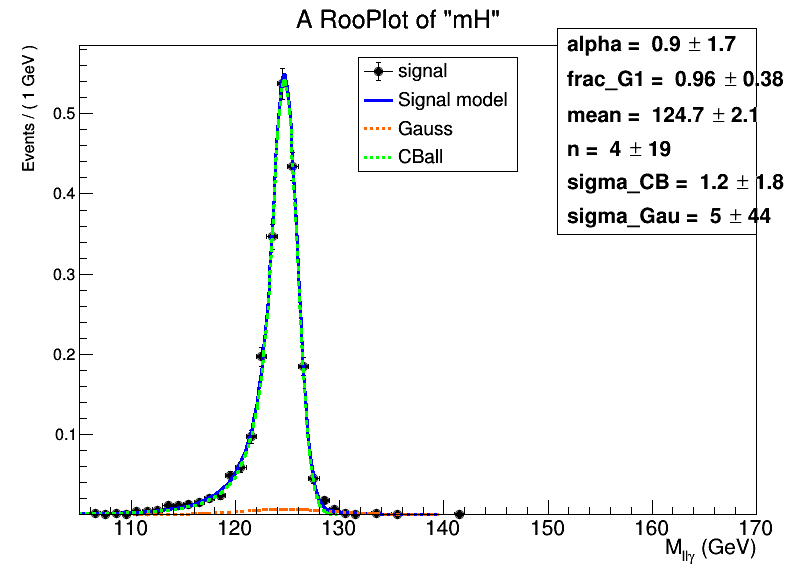
\includegraphics[width=0.40\textwidth]{fig/signal_fit/2016/sigfit_ele_ggF_1_125.png}
		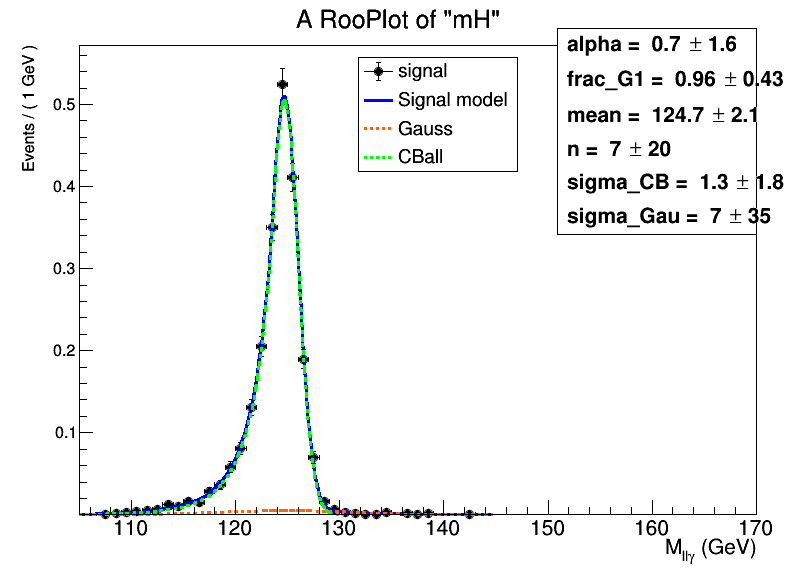
\includegraphics[width=0.40\textwidth]{fig/signal_fit/2016/sigfit_ele_ggF_2_125.png}\\
		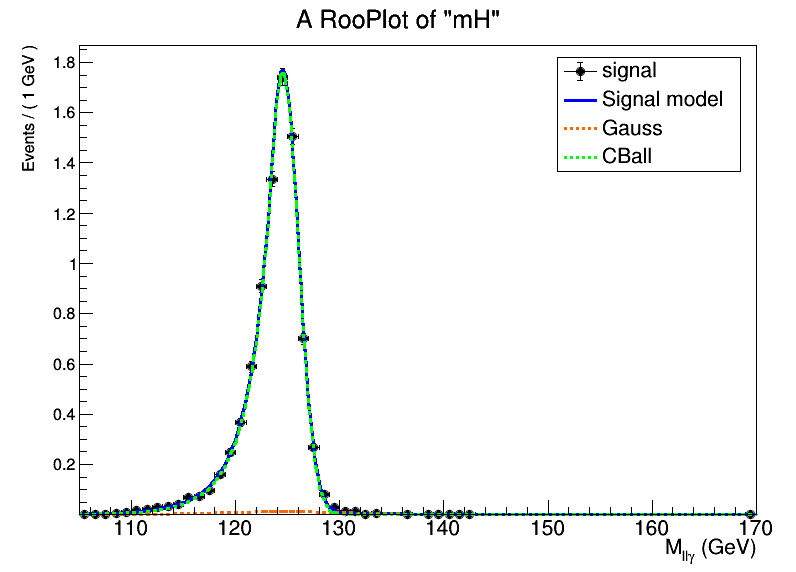
\includegraphics[width=0.40\textwidth]{fig/signal_fit/2016/sigfit_ele_ggF_3_125.png}
		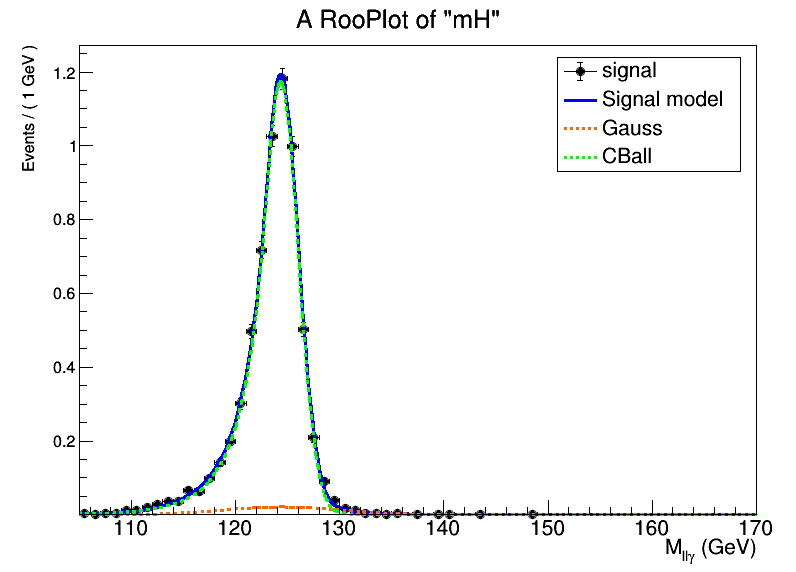
\includegraphics[width=0.40\textwidth]{fig/signal_fit/2016/sigfit_ele_ggF_4_125.png}\\
		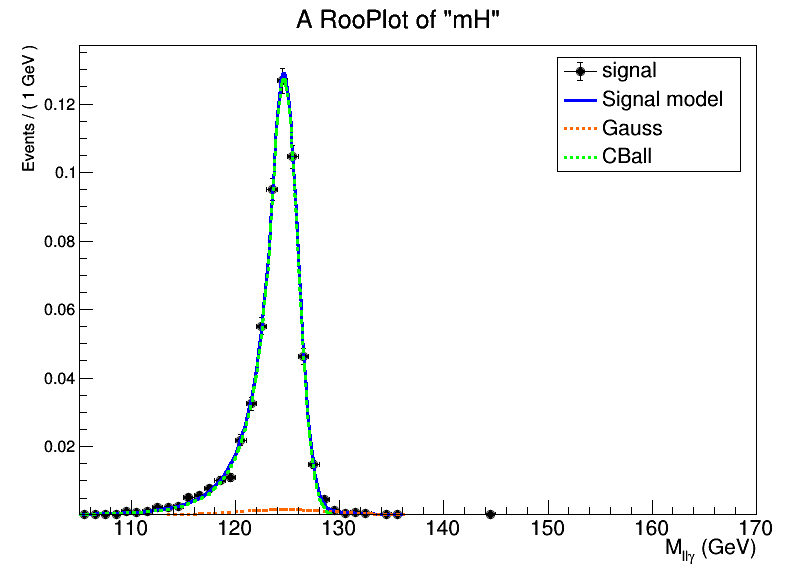
\includegraphics[width=0.40\textwidth]{fig/signal_fit/2016/sigfit_ele_VBF_501_125.png}
		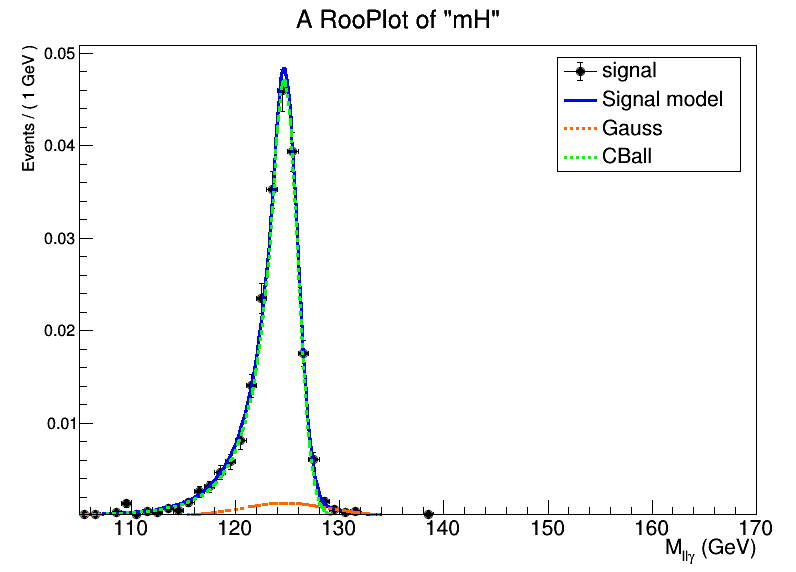
\includegraphics[width=0.40\textwidth]{fig/signal_fit/2016/sigfit_ele_VBF_502_125.png}\\
		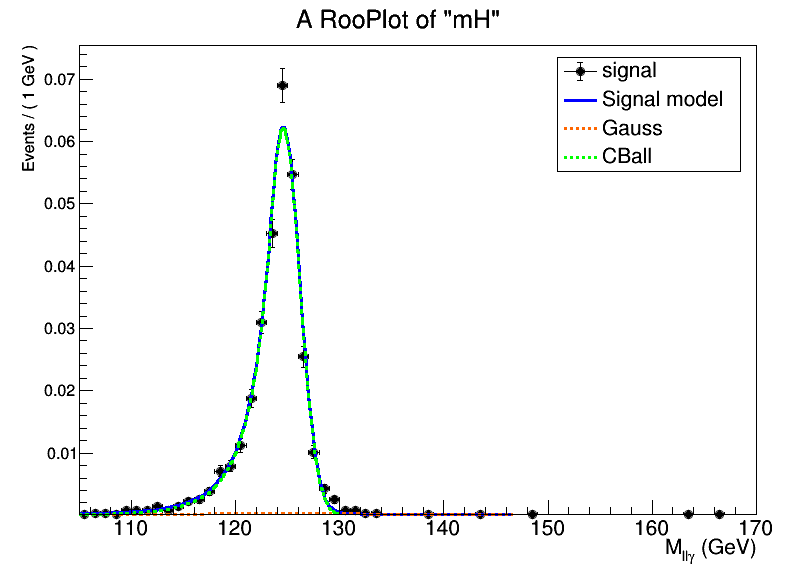
\includegraphics[width=0.40\textwidth]{fig/signal_fit/2016/sigfit_ele_VBF_503_125.png}\\
		\caption{Fits to simulated $m_{\ell^+\ell^-\gamma}$ signal distributions in the electron channel for
            		 $m_\PH=125\GeV$ for the 2016 data-taking period.
			 The blue line shows the total fit function, the green line shows the Crystal Ball function component, and the red line shows the Gaussian function component.
			 The top four plots correspond to the untagged categories, and the bottom three plots correspond to the dijet categories.}
		\label{fig:elesigfit}
	\end{center}
\end{figure}

\begin{figure}
	\begin{center}
		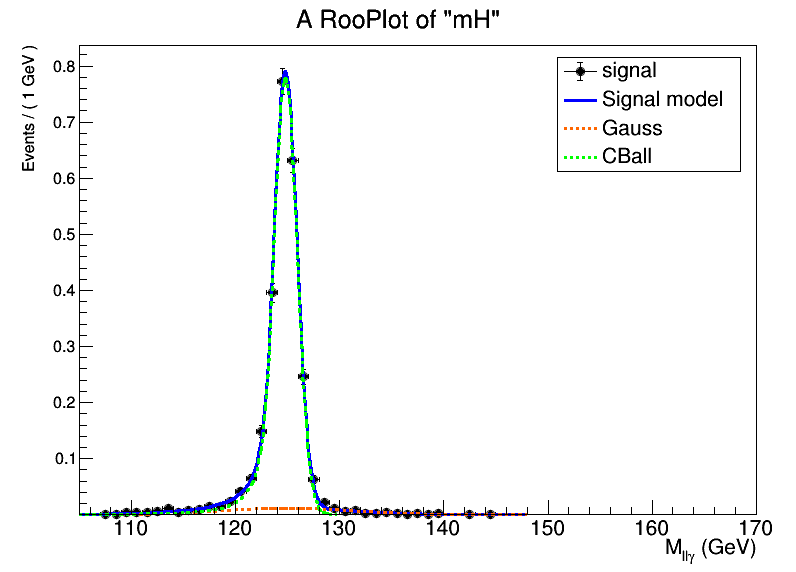
\includegraphics[width=0.40\textwidth]{fig/signal_fit/2016/sigfit_mu_ggF_1_125.png}
		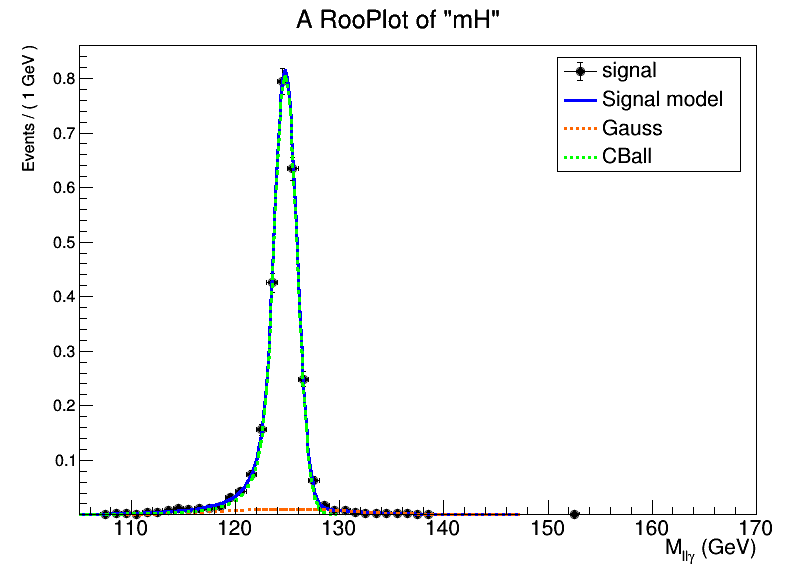
\includegraphics[width=0.40\textwidth]{fig/signal_fit/2016/sigfit_mu_ggF_2_125.png}\\
		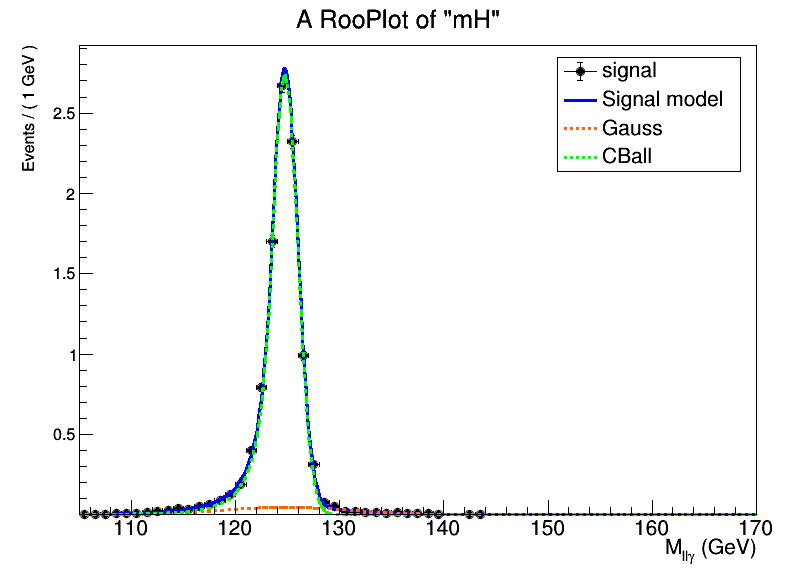
\includegraphics[width=0.40\textwidth]{fig/signal_fit/2016/sigfit_mu_ggF_3_125.png}
		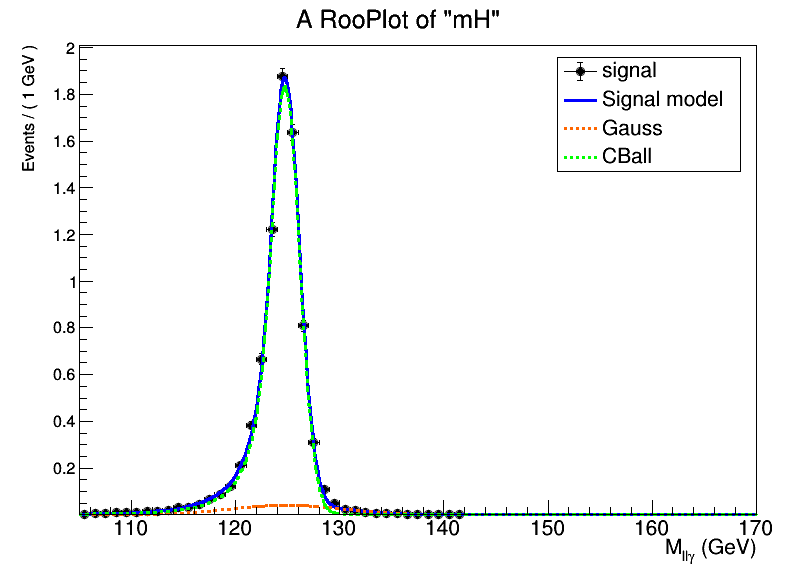
\includegraphics[width=0.40\textwidth]{fig/signal_fit/2016/sigfit_mu_ggF_4_125.png}\\
		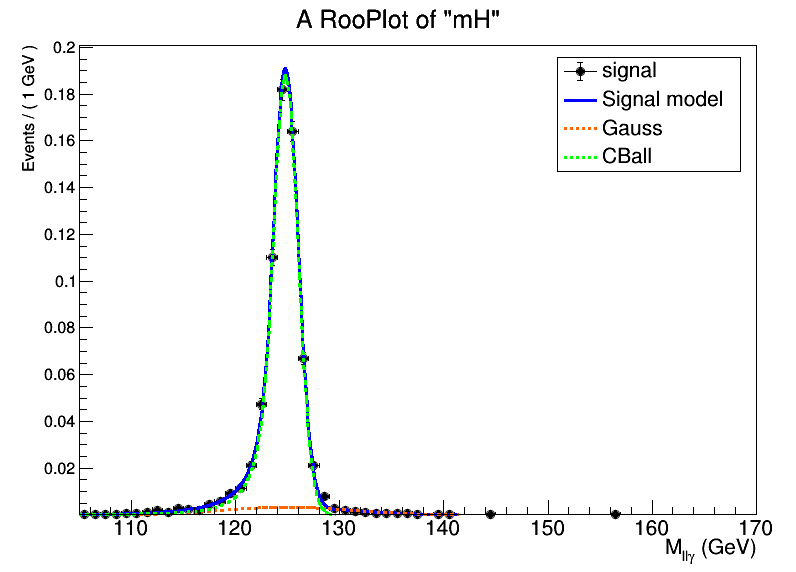
\includegraphics[width=0.40\textwidth]{fig/signal_fit/2016/sigfit_mu_VBF_501_125.png}
		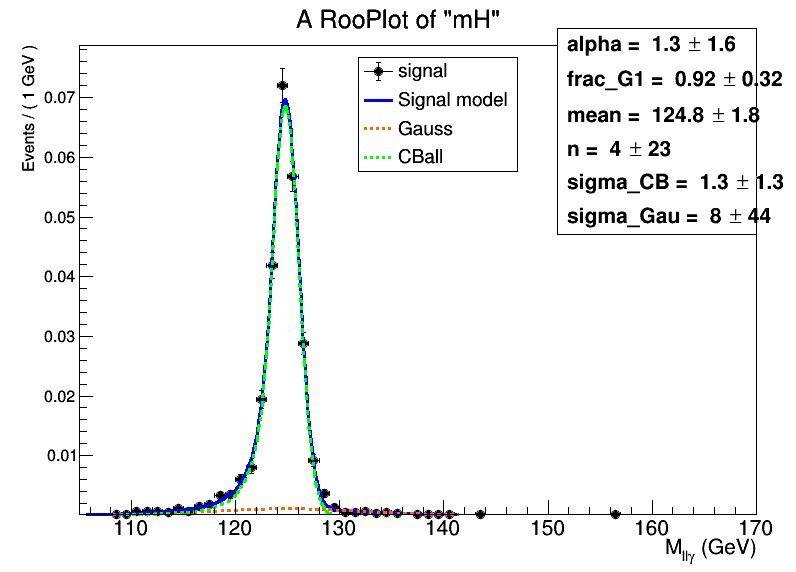
\includegraphics[width=0.40\textwidth]{fig/signal_fit/2016/sigfit_mu_VBF_502_125.png}\\
		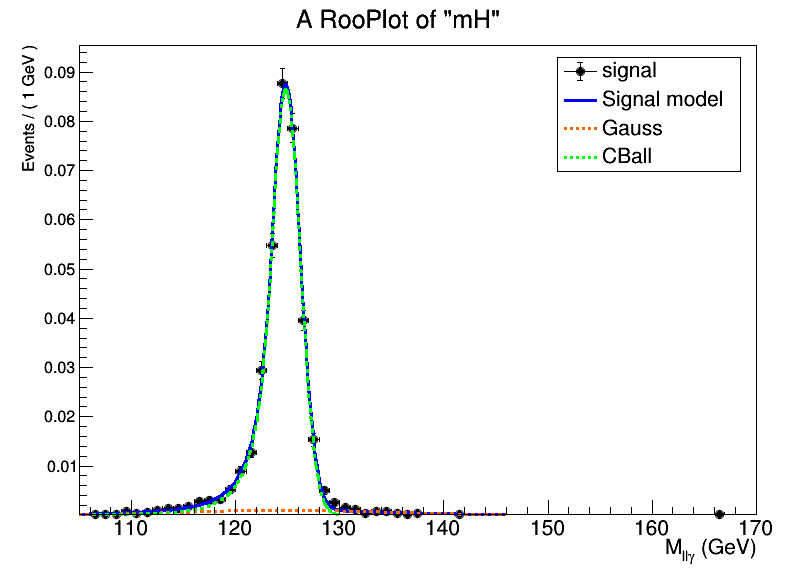
\includegraphics[width=0.40\textwidth]{fig/signal_fit/2016/sigfit_mu_VBF_503_125.png}\\
		\caption{Fits to simulated $m_{\ell^+\ell^-\gamma}$ signal distributions in the muon channel for
            		 $m_\PH=125\GeV$ for the 2016 data-taking period.
			 The blue line shows the total fit function, the green line shows the Crystal Ball function component, and the red line shows the Gaussian function component.
			 The top four plots correspond to the untagged categories, and the bottom three plots correspond to the dijet categories.}
		\label{fig:elesigfit}
	\end{center}
\end{figure}

\begin{figure}
	\begin{center}
	  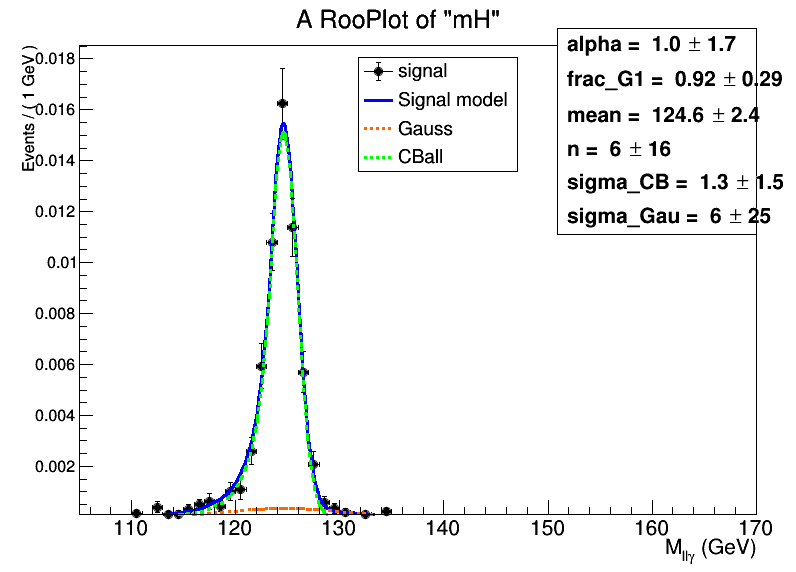
\includegraphics[width=0.40\textwidth]{fig/signal_fit/2016/sigfit_ele_mu_ZH_6789_125.png}
	  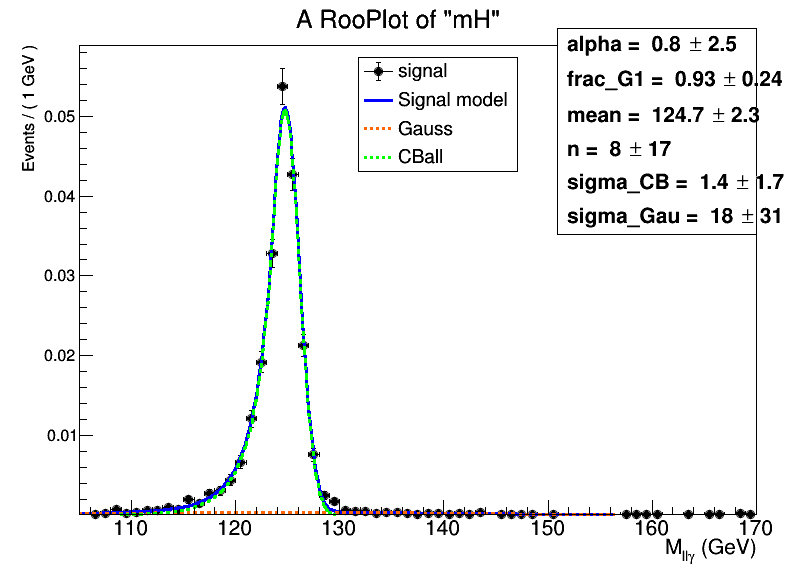
\includegraphics[width=0.40\textwidth]{fig/signal_fit/2016/sigfit_ele_mu_WH_6789_125.png}
		\caption{Fits to simulated $m_{\ell^+\ell^-\gamma}$ signal distributions in the electron and muon channels combined in the lepton-tagged category for
            		 $m_\PH=125\GeV$ for the 2016 data-taking period.
        		 The left plot shows the fit to simulated ZH production events, and the right plot shows the fit to simulated WH production events. 
			 The blue line shows the total fit function, the green line shows the Crystal Ball function component, and the red line shows the Gaussian function component.}
		\label{fig:elemusigfit}
	\end{center}
\end{figure}

\subsection{Resonant Background Modeling}
